\chapter{Opisz eksperymentu}
\section{Układ pomiarowy}
Układ pomiarowt składał się z:
\begin{itemize}
\item Komputera z systemem Linux (Ubuntu) --- wymagany jest, aby na komputerze zainstalowany był język Python wraz z bibliotekami:
matplotlib, numpy, PyQt5. Do sterowania sprzętem wymagane są uprawnienia administratora..
\item Zasilacza diód laserowych firmy Thorlabs model LDC4005 ~\cite{Ldc_book}--- zapewnia stabilne zasilanie prądowe laserab prądem do 5\,A.
Możliwe jest zasilanie ciągłe i impulsywne. Posiada interfejsem SCPI ~\cite{Ldc_book_prog}, umożliwiający sterowanie za pomocą komputera przez USB.
\item Miernik mocy firmy Thorlas firmy Thorlabs model PM100 ~\cite{Pm100_book} --- stworzony do mierzenia mocy wyjściowej z lasera. Pozwala operować na
długościach fali od 400\,nm do 1100\,nm. Posiada interfejsem SCPI ~\cite{Pm100_book}, umożliwiający sterowanie za pomocą komputera przez USB.
\item Kontroler temperatury diod laserowych firmy Thorlabs--- precyzyjny kontroler temperatury pozwalający na zmiany temperatury
chłodniczy lasera podczas operowania prądami do 2\,A.
\end{itemize}
\begin{figure}
\center
  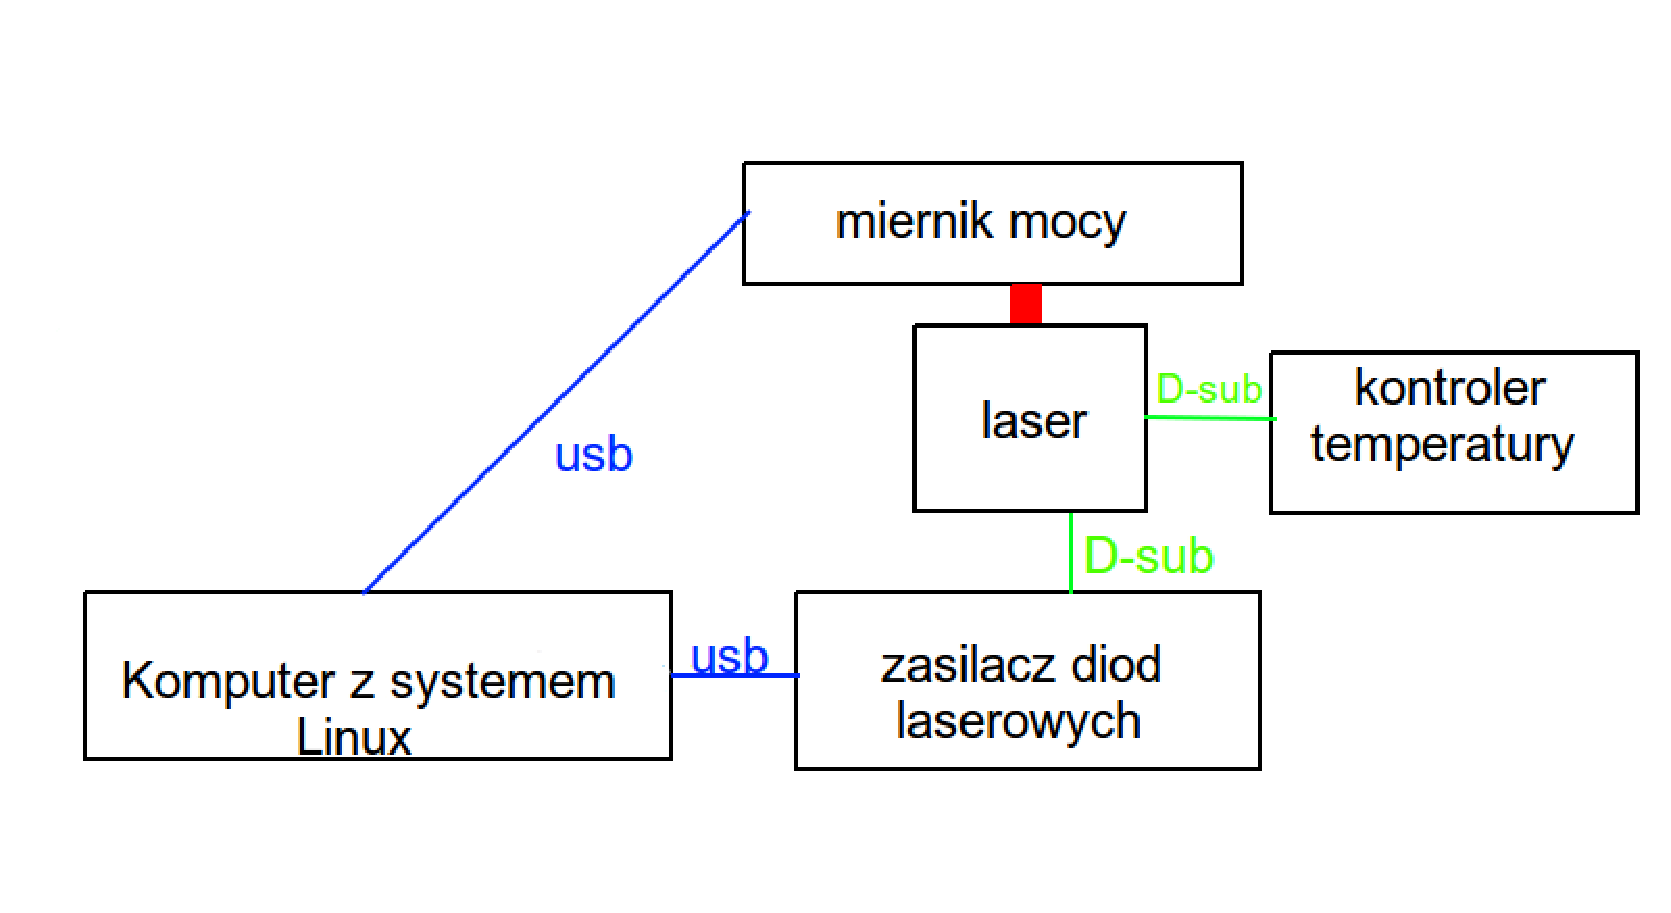
\includegraphics[scale=0.35]{schemat.eps}
  \label{rys1}
  \caption{Schemat układu pomiarowego.}
\end{figure}
\subsection{Przebieg pomiarów}
Laser był umieszczony w mocowaniu diod laserowym połączonych z zasilaczem diod laserowych oraz kontrolerem temperatury.
Na wyjściu lasera umieszczony był miernik mocy. Komunikacja z zasilaczem oraz miernikiem odbywała się za pomocą standardu
komend SCPI przez połączenie USB. Temperatura była zmieniana manualnie na kontrolerze temperatury.
Charakterystyki wyjściowe (czyli wartości prądu zasilania, napięcia na laserze oraz mocy wyjściowej)
mierzone były pod falą ciągła prądu. Wyniki zapisywane były w pliku tekstowym.